



\subsection*{Sources of Inspiration}

The development of the game engine draws inspiration from several established platforms:

        \textbf{Unity:} The math engine draws inspiration from Unity's advanced mathematical computations and transformations, leading to the development of a robust internal framework.


    % 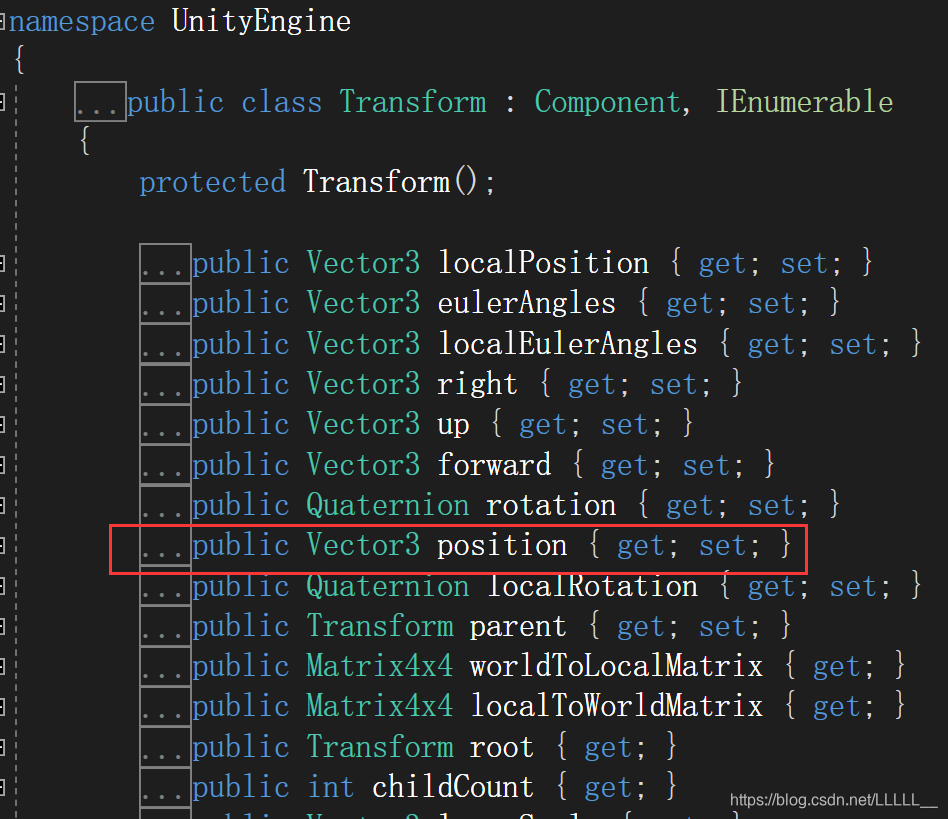
\includegraphics[height=5cm]{unity_transform}
    % \caption*{Unity Transform}

 \begin{lstlisting}
  void start();
  void update();
  int main() { Awake(); }
  void Awake() {
    RenderEngine::setStart(start);
    RenderEngine::setUpdate(update);
    RenderEngine::setFixedUpdate(fixedUpdate);
    // 
    RenderEngine::START(true);
  }
  void start() {
    Gameobject go;
    go.transform.position = Random::Vector3().normalised *  Random::Value(-5, 5); 
    Debug::Log(go.transform.position)
  }
  \end{lstlisting}


% \begin{figure}[htbp]
%     \centering
%     \begin{minipage}[t]{0.4\textwidth}
%         \textbf{Unity:} The math engine is inspired by Unity's robust handling of complex mathematical computations and transformations. Unity's versatility and efficient math libraries have guided the development of our own mathematical framework within the engine.
%     \end{minipage}\hfill
%     \begin{minipage}[t]{0.4\textwidth}
%         \centering
%         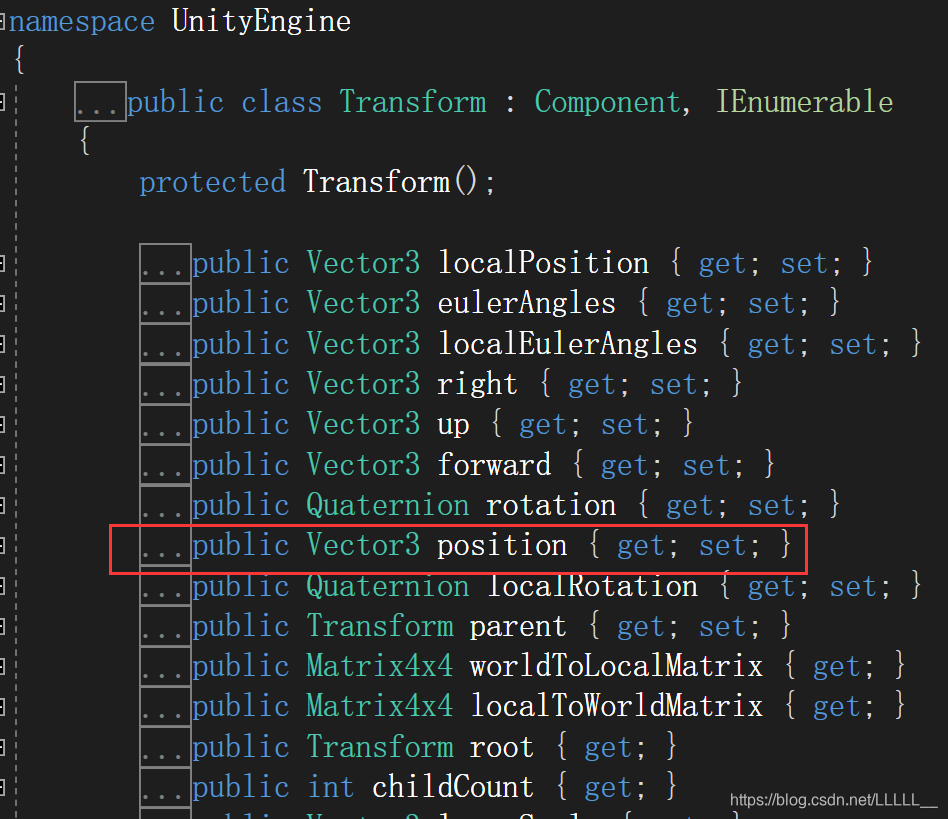
\includegraphics[height=5cm]{unity_transform}
%         \caption*{Unity Transform}
%     \end{minipage}
%     
%     \begin{minipage}{0.45\textwidth}
%         \begin{lstlisting}[language=C++, caption={Example Code}]
% void start();
% void update();
% int main() { Awake(); }
% void Awake() {
%   RenderEngine::setStart(start);
%   RenderEngine::setUpdate(update);
%   RenderEngine::setFixedUpdate(fixedUpdate);
%   // 
%   RenderEngine::START(true);
% }
% void start() {
%   GameObject go;
%   go.transform.position = Random::Vector3().normalized() * Random::Value(-5, 5); 
%   Debug::Log(go.transform.position);
% }
%         \end{lstlisting}
%     \end{minipage}
% \end{figure}


\textbf{p5.js:} The rendering engine draws inspiration from p5.js, renowned for its simplicity and accessibility in the creative coding community. The straightforward approach to rendering and graphical output in p5.js has influenced our rendering pipeline's design, making it powerful and user-friendly.













\begin{lstlisting}

  point(x, y, c); // Changes the color of the pixel at location <x, y> to c

  line(<<x>, <y>>, 
       <<x>, <y>>); // Draws a line between 2 points

  background(color);

  square(point1, point2);
  fill(color);
  noStroke();
  circle(point , radius);

\end{lstlisting}








% \begin{lstlisting}
% void start();
% void update();
% int main() { Awake(); }
% void Awake() {
%   RenderEngine::setStart(start);
%   RenderEngine::setUpdate(update);
%   RenderEngine::setFixedUpdate(fixedUpdate);
%   // MUST BE CALLED LAST
%   RenderEngine::START(true);
% }
% void start() {
%   Gameobject go; int speed = 0.01;
%   Debug::Log(go.transform.name)
%   Debug::Log(go.transform.position)
%   
%   go.transform.translate(Vector3::Right * speed)
%   Debug::Log(go.transform.position)
%   go.transform.position = Vector3::one * Math::sqrt(Math::pi);
%   Debug::Log(go.transform.position)
% }
% \end{lstlisting}









